% !TEX root = document.tex

\lstdefinestyle{mystyle_bt_basic}{
language = Python,
otherkeywords = {E, Null, 0, 1, 2, 3, 4, 5, 6},
keywordstyle = [2]{\color{num_color}},
morekeywords = [2]{0, 1, 2, 3, 4, 5, 6}
}
\lstdefinestyle{mystyle_bt_basic_stratego}{
language = Python,
otherkeywords = {r-zero, 0},
morekeywords = {E, Exp, Null, program},
keywordstyle = [2]{\color{num_color}},
morekeywords = [2]{0},
keywordstyle = [3]{\color{kw_alt}},
morekeywords = [3]{constructors, rules, strategies, topdown, Int}
}
\lstdefinestyle{mystyle_increment_comparison}{
language = Python,
otherkeywords = {r-increment5, r-increment1},
morekeywords = {E, S, program},
keywordstyle = [2]{\color{kw_alt}},
morekeywords = [2]{rules, strategies, topdown}
}
\lstdefinestyle{mystyle_copy_up}{
language = Python,
otherkeywords = {r-copy-up},
morekeywords = {E, Null}
}

\chapter{Introduction}
\label{chap:introduction}
Traversing and transforming tree-like data structures is a common occurrence in developing program analysis tools, refactoring tools, and compilers or interpreters that operate on abstract syntax trees (AST's). Control over the application order of the transformations, the propagation of effects, and the traversal of the input data is often necessary to correctly implement more complex program transformations\autocite{LaemmelVV02}. Most programming paradigms provide limited support for separating traversal control from the rest of the program, limiting reusability and scalability\autocite{LaemmelVV02}.

Strategic programming languages address this challenge by separating the transformations that are performed from the manner in which trees are traversed. Users define rewrite rules that operate on trees, and strategies that determine how trees are traversed and when rewrite rules are applied. These strategies are also generic in the sense that they are polymorphic: a single definition of the strategy is enough to work on any type of node \autocite{LaemmelVV02, Visser01}.

In more complex programs operating on tree-like data structures, multiple traversals are often performed on the same tree, leading to potentially unnecessary repeated visits of nodes. Identifying traversals that can be fused together safely reduces repeated visits and thus runtime overhead. This optimization is called traversal fusion.

Strategic programming languages, while intuitive and convenient to use in their domains, are high-level languages. The trade-off between convenient abstractions in high-level languages and computational performance in low-level languages is well-established \cite{SiskindP16a, Kovacs24}. At the same time, optimizing compilers can, in some cases, recover performance in high-level languages \cite{Mainland17}, and in many cases programs written in higher-level languages ``rely heavily on [these] optimizations to achieve adequate performance" \cite{Kovacs24}. In recent times, as Moore's law is seemingly coming to an end while Artificial Intelligence (AI) creates increasingly large performance demands, compiler optimizations may be more relevant than ever \cite{ZHANG2023}. Only  a small number of compiler optimizations are available for strategic languages, and these languages suffer from a general lack of research on how to improve their performance compared to more popular paradigms. We contribute to this problem by attempting to apply the traversal fusion optimization in strategic programming.

The number of fusion opportunities, as well as the amount of runtime overhead due to repeated visits, depend on the program being analyzed and can vary significantly between different programs. A program could theoretically have no fusion opportunities at all, or arbitrarily many. The best-case scenario for the traversal fusion optimization is a program with a large number of traversals that perform different, non-conflicting operations. The possible performance increase due to traversal fusion further depends on the input size. The traversal fusion optimization is ideal for tree traversal programs that are compiled once and then run on many different inputs, such as program transformation tools. In such a scenario, the increased compile time is a one-time investment that can, in a sense, be amortized over all subsequent executions of the program. Previous work on imperative programs has shown that traversal optimization is effective for real-world program transformation use cases: Grafter can achieve speedups between 1.5 and 4.5 times in a render tree transformation benchmark, with larger input sizes achieving a greater speedup \cite{SakkaS017, SakkaSN019}. 

However, this is no guarantee that the optimization is effective for strategic programming. Even if the same analysis can be performed, and the same fused traversal implemented, strategic languages have different data representations, different ways of implementing traversals, and different sources of overhead. If it is effective in strategic programming, we hope that it could be one of many optimizations that gradually increase the performance of strategic programming languages and consequently increase the adaptation of the paradigm.

\section{Stratego}
In this thesis, we focus mainly on the strategic programming language Stratego, originally developed around 2001 \autocite{Visser01}, and currently still in development at the Delft University of Technology. Stratego allows users to specify rewrite rules, strategies, and input data in Annotated Terms (ATerms). ATerms are a simple and efficient way to represent tree-like data structures \autocite{BrandJKO00}.

As an example, consider the binary tree of integers and its ATerm representation shown in \autoref{fig:binary-tree-basic}, as well as \autoref{fig:binary-tree-basic-stratego}, which shows how to define such a tree in Stratego, and how to perform a basic operation on it.

\begin{figure}
\centering

\begin{subfigure}{0.5\textwidth}
    \centering
    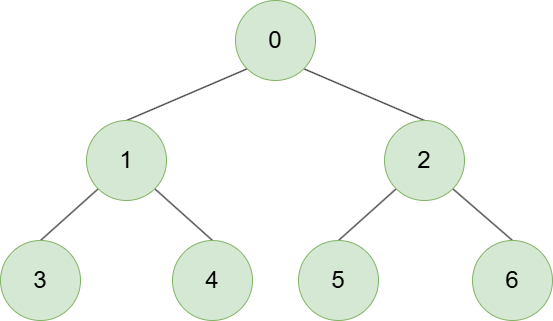
\includegraphics[width=6cm]{./img/binary-tree-basic.png}
    \subcaption{Binary tree of integers}
\end{subfigure}%
\begin{subfigure}{0.5\textwidth}
\centering
\begin{lstlisting}[style=mystyle_bt_basic]
    E(0,
      E(1,
        E(3, Null(), Null()), E(4, Null(), Null())
      ),
      E(2,
        E(5, Null(), Null()), E(6, Null(), Null()
      )
    )
\end{lstlisting}
    \subcaption{ATerm representation}
\end{subfigure}

\caption{A binary tree of integers and its ATerm representation.}
\label{fig:binary-tree-basic}
\end{figure}

To define a binary tree the constructors \texttt{E} and \texttt{Null} are defined. The constructor \texttt{E} represents nodes that contain an integer, and that have two children that are also \texttt{E} nodes, or \texttt{Null} if the node is a leaf.

\begin{figure}
\begin{lstlisting}[style = mystyle_bt_basic_stratego]
    constructors
      E: Int * Exp * Exp -> Exp
      Null: Exp

    rules
      r-zero:
        E(v, l, r) -> E(0, l, r)

    strategies
      program = topdown(r-zero)
\end{lstlisting}
\caption{A binary tree and an operation on it, defined in Stratego.}
\label{fig:binary-tree-basic-stratego}
\end{figure}

As an example of an operation that can be performed on this tree, a rewrite rule is defined in \autoref{fig:binary-tree-basic-stratego} that sets the value of every node to zero. This rule sets the first child (the \texttt{v} field) to 0, but does not recursively apply itself to the children \texttt{l} and \texttt{r}. Instead, this traversal logic is factored out of the rule into a generic traversal. To apply this rule to the entire tree, all we have to do is call the \texttt{topdown} strategy. The \texttt{topdown} strategy takes a rule, applies it to the current node, and then applies it to each of that node's children recursively and generically. 

\texttt{topdown} is just one of many available strategies in Stratego, and users can also define their own strategies. This small example already shows one of the main benefits of strategic programming: adding a new type of constructor to this tree would not require any changes to the traversal logic, unless different behavior was specifically desired for that constructor.

\section{Traversal Fusion}
In Stratego, users can easily write programs consisting of sequences and combinations of traversals that can perform complex operations on trees. This is quite useful: for example, a user might simply want to apply a set of rules to a tree, and then another set, and then another. This can be expressed naturally in just a few lines of code. Or, consider a program transformation that performs a simplification: applying such a rule once may introduce new opportunities for simplification. Thus, such a rule might have to be applied repeatedly until the tree no longer changes.

However, the ease with which more traversals can be added into a Stratego program does raise the question of whether this is always efficient. Consider applying a single rule top-down multiple times in a row on the same tree. It is very easy to simply call \texttt{topdown} multiple times. But in some cases it might also be possible to change the rewrite rule itself to still do everything in a single traversal. As the input data get larger, the traversals themselves start taking up a considerable amount of the program runtime through memory accesses. Performing fewer traversals would reduce the number of times nodes are visited, and thus also the number of memory accesses. For very large input data, reducing the number of unique node visits also reduces cache misses, which have a significant performance impact. In theory, then, performing fewer traversals should be faster.

This means that users, especially when writing more complex programs, do have to think about how their rewrite rules and traversals interact. This seems somewhat counter to the objective of strategic programming languages to separate these things. In many cases, the version of a program with fewer traversals might also be more complex or less intuitive to write. As such, automatically identifying opportunities for traversal fusion is an interesting and promising optimization for strategic programming. It is important to note that traversal fusion does \textit{not} change the rewrite rules, and achieves fusion in a different way. The time savings come from the reduction in overhead created by the memory accesses of the traversals. Fewer traversals after fusion lead to less overhead.

\subsection{Example of Legal and Illegal Fusion}
Consider the example shown in \autoref{fig:increment-by-five-comparison}. In this example, we want to apply a rule that increments the values in a binary tree of integers by five. This can be done efficiently in a single top-down traversal applying a single rewrite rule that increments the values by five (\autoref{fig:increment-by-five-comparison-1}). It can also be done by performing five top-down traversals in a row, each applying a rewrite rule that increments values by one (\autoref{fig:increment-by-five-comparison-2}). The traversal fusion optimization would analyze the latter program and determine that these five traversals can safely be fully fused together. In this case, a program that only goes through the tree top-down once, applying the rewrite rule five times in a row at every node, has equivalent behavior (\autoref{fig:increment-by-five-comparison-3}).

\begin{figure}

\begin{subfigure}{\textwidth}
\begin{lstlisting}[style = mystyle_increment_comparison]
    rules
      r-increment5 :
        E(v, l, r) -> E(S(S(S(S(S(v))))), l, r)
    
    strategies
      program = topdown(r-increment5)
\end{lstlisting}
\subcaption{Single traversal, with a single rewrite rule}
\label{fig:increment-by-five-comparison-1}
\end{subfigure}

\begin{subfigure}{\textwidth}
\begin{lstlisting}[style = mystyle_increment_comparison]
    rules
      r-increment1 :
        E(v, l, r) -> E(S(v), l, r)
    
    strategies
      program = topdown(r-increment1); topdown(r-increment1);
        topdown(r-increment1); topdown(r-increment1); topdown(r-increment1)
\end{lstlisting}
\subcaption{Five traversals}
\label{fig:increment-by-five-comparison-2}
\end{subfigure}

\begin{subfigure}{\textwidth}
\begin{lstlisting}[style = mystyle_increment_comparison]
    rules
      r-increment1 :
        E(v, l, r) -> E(S(v), l, r)
    
    strategies
      program = topdown(r-increment1; r-increment1;
        r-increment1; r-increment1; r-increment1)
\end{lstlisting}
\subcaption{Single traversal, fused from five traversal version}
\label{fig:increment-by-five-comparison-3}
\end{subfigure}

\caption{Comparison of increment-by-five programs.}
\label{fig:increment-by-five-comparison}
\end{figure}

Finding fusion opportunities is not always this simple. As seen in the previous example, consecutive traversals writing to the same field does not necessarily prevent fusion. Problems generally arise when traversals use information stored in nodes \textit{other} than the current node. The intuitive reasoning behind this is that traversal fusion alters a program's execution order, and other nodes may be in invalid states. For example, when executing the fused increment program, the current node may have a value of $5$, while its children all sit at $0$. In the unfused program that performs five traversals, values never differ by more than $1$.

As a concrete example of when fusion is not legal, define a rewrite rule that copies the value of a node's child into that node, as shown in \autoref{fig:twotd-counterexample-1}.

\begin{figure}

\begin{subfigure}{\textwidth}
\begin{lstlisting}[style = mystyle_copy_up]
    r-copy-up:
      E(_, E(v, c)) -> E(v, E(v, c))

    r-copy-up:
      E(v, Null()) -> E(v, Null())
\end{lstlisting}
\subcaption{\texttt{copy-up} rewrite rule}
\label{fig:twotd-counterexample-1}
\end{subfigure}

\begin{subfigure}{0.5\textwidth}
\centering
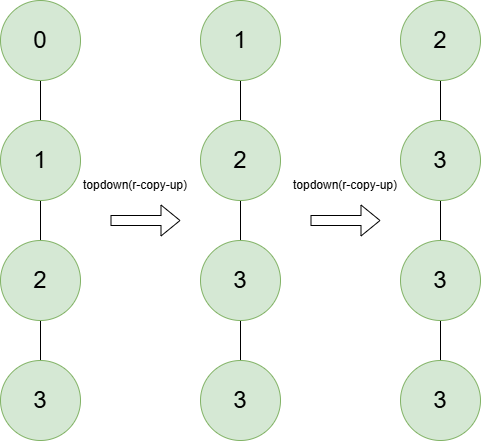
\includegraphics[width=6.5cm]{./img/twotd-counterexample-unfused.png}
\subcaption{Two top-down traversals in a row}
\label{fig:twotd-counterexample-2}
\end{subfigure}%
\begin{subfigure}{0.5\textwidth}
\centering
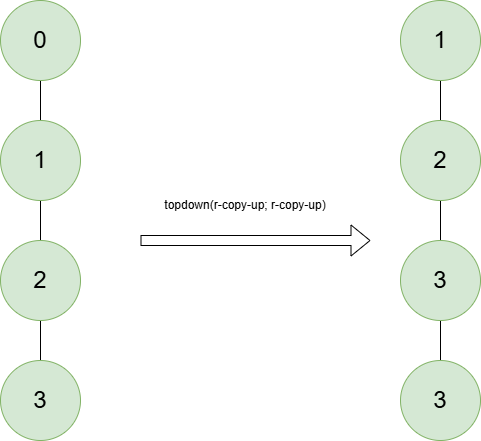
\includegraphics[width=6.5cm]{./img/twotd-counterexample-fused.png}
\subcaption{Single top-down traversal}
\label{fig:twotd-counterexample-3}
\end{subfigure}

\caption{Counter-example to the fusion of two top-down traversals.}
\label{fig:twotd-counterexample}
\end{figure}

Executing this rule twice top-down on an example tree gives the result shown in \autoref{fig:twotd-counterexample-2}. However, fusing the top-down traversals into a single top-down traversal results in \autoref{fig:twotd-counterexample-3}, which is not the same. The intuition here is that the second application of the rewrite rule in the fused version does not actually do anything. It simply copies up the value of the child again, but that value cannot have changed. In the unfused version, that value \textit{has} changed (except in the case of the leaf), because the rewrite rule has already been applied once to that child.

\section{This Thesis}
Using information stored in other nodes does not always prevent fusion. Determining when it (or another effect) does and does not prevent fusion is exactly the problem of automated traversal fusion. Traversal fusion is not a totally new concept, and some research has been done on this topic. For example, research has been done on very specific fusions in Stratego that are always possible \autocite{JohannV01}. More general traversal fusion has also been achieved in other contexts, for example with circular programming \autocite{FernandesPS07}, or using dependency analysis \autocite{SakkaS017, SakkaSN019}. We will focus on the dependency analysis approach in this thesis. Other related work is discussed in more detail in \autoref{chap:rw}.

None of the research that has been done, however, applies directly to strategic programming and fusing generic traversals. It is not clear whether this can be done at all in strategic programming, how it might be done, and what its potential benefit might be.

The research question for this thesis is: `Can generic traversal fusion be performed in strategic programming languages, and what is the impact of this optimization on strategic programs?'

We make the following contributions in this thesis:
\begin{itemize}
    \item We develop an algorithm that can apply the traversal fusion optimization in strategic programming languages based on the TreeFuser and Grafter algorithms\cite{SakkaS017, SakkaSN019}. It can analyze the dependencies of a set of traversals and rewrite rules, and synthesize a fused traversal if one exists.
    \item We implement a proof-of-concept (POC) traversal fusion optimizer using this algorithm that works on a subset of the Stratego language. This POC supports simple constructors (e.g. no list types), rewrite rules without side effects (function calls are allowed), and a single sequence of operations consisting of any combination of calls to \texttt{all}, rule applications, calls to \texttt{topdown} or \texttt{bottomup}, or calls to other strategies using only these features.
    \item We evaluate the POC on a synthetic benchmark simulating the rendering of a web page to determine the real benefit of this optimization in strategic programming. We find that it effectively reduces node visits by over 40\%, while not having measurable impact on runtime or memory usage. While a runtime improvement is technically present, it is caused by our code synthesis and not the fusion. Under some circumstances (e.g. when performing full fusion), traversal fusion can have a measurable performance impact in strategic programming, but these situations are less likely to occur in real-world usage.
\end{itemize}